\documentclass{beamer}
\usetheme{Oxygen}
\usepackage{verbatim}
\usepackage{minted}

\title{Automated Code Transformation for Distributed Training of TensorFlow ML Models}
\author{Yusung Sim\inst{1}, Wonho Shin\inst{1}, Sungho Lee\inst{2}}
\institute{
  \inst{1}%
  School of Computing, KAIST
  \and
  \inst{2}%
  Department of Computer Science and Engineering, Chungnam National University
}
\date{2022}

\begin{document}
% 0. Title
\frame{\titlepage}


% 1. Introduction
\begin{frame}{Reducing ML Training Time}
  Reducing the \textbf{training time} is important factor in ML developement.\\

  \begin{itemize}
    \item Simple CNN-based classifier for MNIST trains in 2$\sim$3 hours
    \item Training BERT model in single TPU takes over 1.5 month
  \end{itemize}

  Long training time makes CI/CD infeasible.
  \begin{itemize}
    \item Training data increases largely in real time
    \item TODO: summarize this frame with good diagram
  \end{itemize}
\end{frame}


\begin{frame}{Distributed ML Training}
  \begin{definition}
    \textbf{Distributed training} is a ML training technique
    where the computation is distributed over multiple hardware devices
    (GPUs, TPUs, etc.). It reduces the total training time,
    ideally inverse-proportional to the device number.
  \end{definition}

  \textbf{Data-parallel approach} is commonly used.
  \begin{itemize}
    \item Multiple instances of the model assigned to each devices.
    \item Train dataset distributed over device.
    \item Gradients are averaged then applied to the model.
    \item Use \textit{"Synchronous SGD"} optimization.
  \end{itemize}
\end{frame}


\begin{frame}[fragile]{Horvod: Distributed Training Framework}
  Distributed training code is often written in \textbf{Horovod},\\
  a data-parallel distributed training framework for Python. 
  \begin{figure}[!h]
    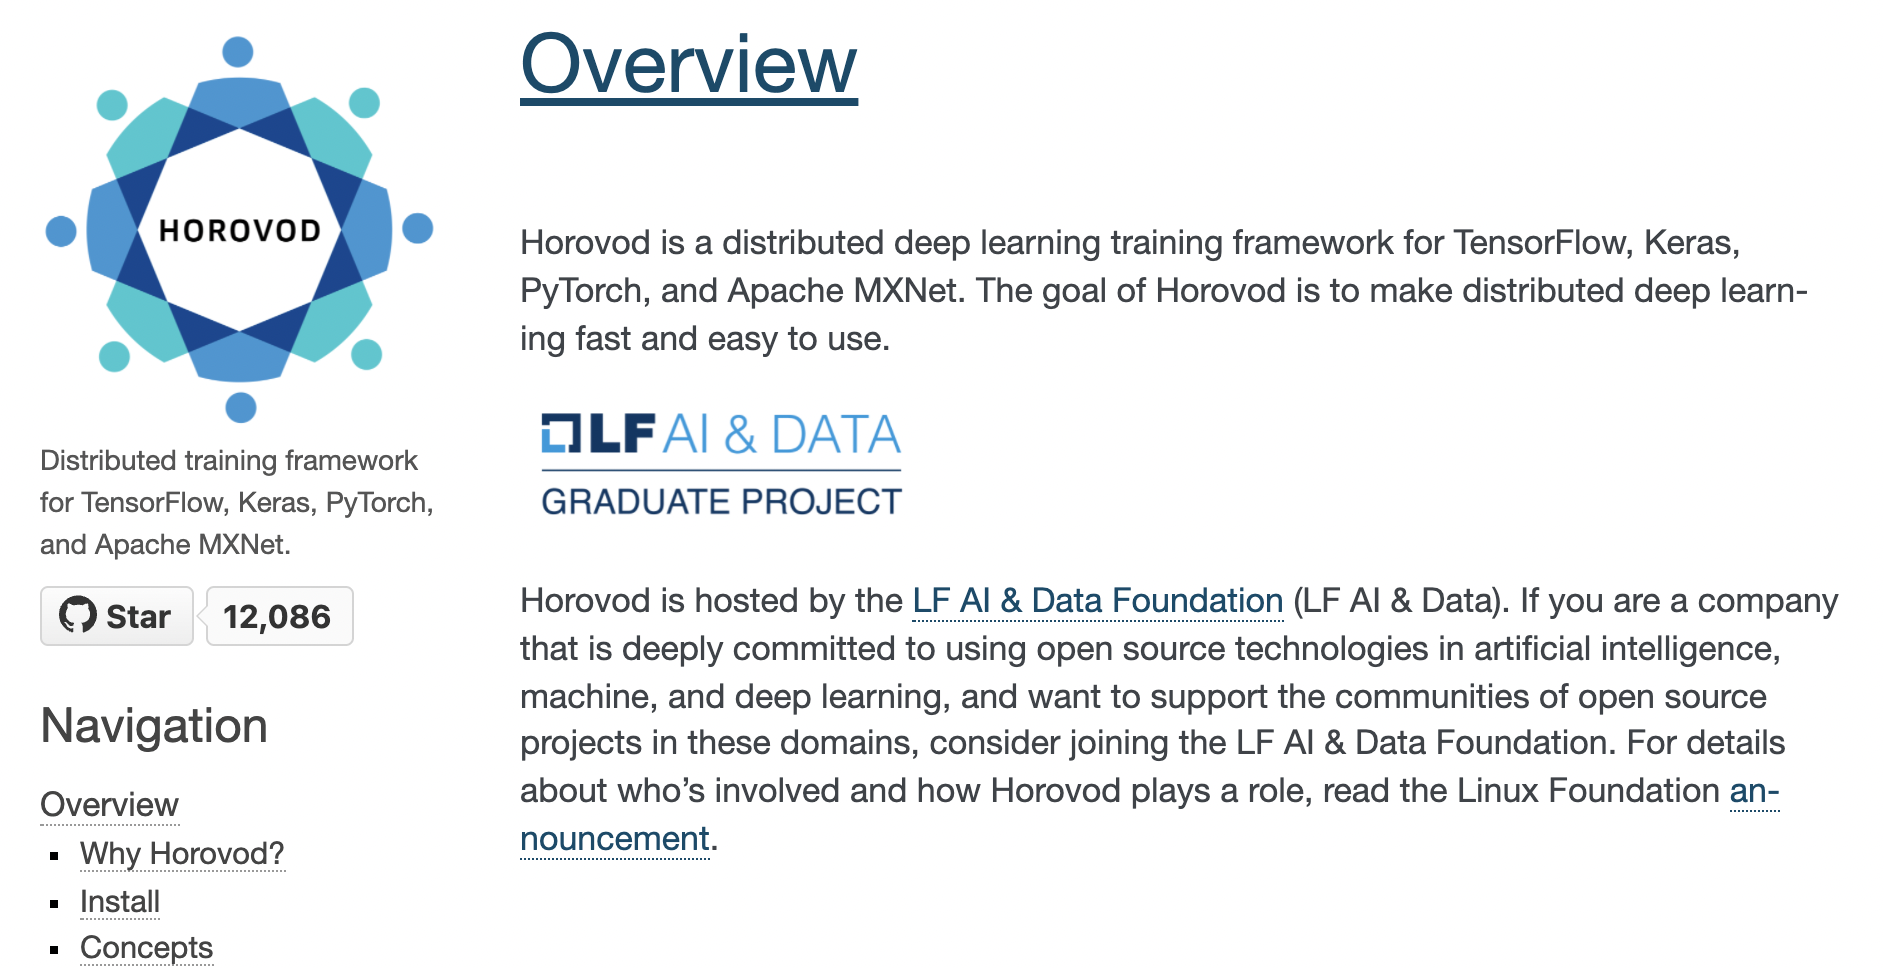
\includegraphics[height=55mm]{horovod_logo}
  \end{figure}
\end{frame}


\begin{frame}{Distributing TensorFlow ML Training Code}
  Explain rewriting single-GPU based training code 
  into distributed training code
\end{frame}


\begin{frame}[fragile]{Rewriting}
% code block
\begin{minted}{Python}
def main():
  print("hello") 
\end{minted}
\end{frame}


\begin{frame}
  \frametitle{Challenge: Rewriting Distributed Training Code}
  \begin{itemize}
    \item Manual rewriting is tedious and time-consuming
    \item Developer must understand distributed training API
    \item Actual code changes are mostly syntactic and simple
  \end{itemize}
\end{frame}


\begin{frame}
  \frametitle{Automatic code transformation}
  Propose automatic code transformation for distributed ML training
  \begin{itemize}
    \item Define formal transformation rule
    \item Implement the rule as a software
  \end{itemize}
\end{frame}


% 3. Method
\begin{frame}
  \frametitle{Formal Code Transformation Rule: Definition}
  Formal definition of code transformation\\
  Function from AST to AST  
\end{frame}


\begin{frame}
  \frametitle{Formal Code Transformation Rule: Environment}
  Environment parameter: store important identifiers
\end{frame}


\begin{frame}
  \frametitle{Formal Code Transformation Rule: Example}
  With example, explain how transform function applies to the code AST
\end{frame}


\begin{frame}
  \frametitle{Training API Pattern}
  Training codes use different APIs to train the model.\\
  Different type of training code shoud be transformed with different rule.\\
  Analyze training API pattern.
\end{frame}


\begin{frame}
  \frametitle{Class Hierarchy Analysis}
  User-defined class inherits TensorFlow classes.\\
  Use CHA to identify such usages
\end{frame}


\begin{frame}
  \frametitle{Implementation}
  Scala, ...
\end{frame}


\begin{frame}
  \frametitle{Evaluation}
  Experiment on 11 selected models.\\
  Transformation succes
  manually checked that they are correctly transformed.\\
\end{frame}

% ----------------------------------------------------

% for record
\begin{frame}[fragile]
  \frametitle{Code example}
  \begin{verbatim}
  def add(x, y):
    return x + y
  \end{verbatim}
\end{frame}

\end{document}
